% CCC Congress talk: RE'ing a 1997 modem with an LLM in the loop.
%
% Build with: make           (slides only)
%             make notes     (slides + speaker notes pages, half-and-half)
%             make handout   (handout mode, no overlays)
%
% A `\notesmode` toggle is set in the wrapper Makefile by passing
% `\PassOptionsToPackage{show notes}{beamer}` via -jobname.

\documentclass[aspectratio=169,11pt]{beamer}

\usetheme{metropolis}
\usepackage{appendixnumberbeamer}
\usepackage[utf8]{inputenc}
\usepackage[T1]{fontenc}
\usepackage{lmodern}
\usepackage{microtype}
\usepackage{listings}
\usepackage{xcolor}
\usepackage{booktabs}
\usepackage{tikz}
\usetikzlibrary{positioning,arrows.meta,fit,backgrounds,calc}
\usepackage{pgfpages}

% Speaker notes — show by default if NOTESMODE is defined externally.
% Build target `make notes` passes \def\notesmode{1} via the command line.
\ifdefined\notesmode
  \setbeameroption{show notes on second screen=right}
\else
  \setbeameroption{hide notes}
\fi

% Code listing style.
\definecolor{codebg}{HTML}{F5F1E8}
\definecolor{codekw}{HTML}{8E2C5A}
\definecolor{codecm}{HTML}{707070}
\definecolor{codestr}{HTML}{2A6A2A}

\lstdefinelanguage{sleigh}{
  morekeywords={define,space,token,is,export,local,goto,return,call,
                if,macro,attach,with,export,unimpl,pcodeop,endian,alignment},
  morecomment=[l]{\#},
  sensitive=true,
  morestring=[b]"
}

\lstdefinelanguage{disasm}{
  morekeywords={SEI,STI,JMP,LDA,LDX,LDY,STA,STX,STY,JSR,RTS,CMP,BNE,BEQ,
                BPL,BMI,BCS,BCC,BVS,BVC,BRA,CLD,CLC,SEC,CLI,SED,
                ADC,SBC,AND,ORA,EOR,ASL,LSR,ROL,ROR,INC,DEC,
                INX,INY,DEX,DEY,TXA,TYA,TAX,TAY,TXS,TSX,
                NOP,BRK,RTI,PHA,PLA,PHP,PLP,PHX,PHY,PLX,PLY,
                ADD,ASR,NEG,LAB,MPY,MPA,RND,CLW,TAW,TWA,
                PSH,PUL,PHW,PLW,EXC,RBA,SBA,BAR,BAS,
                JSB0,JSB1,JSB2,JSB3,JSB4,JSB5,JSB6,JSB7,
                NXT,LII,LAI,LAN,INI,PHI,PLI,PIA,TIP,
                BBR,BBS,RMB,SMB},
  morecomment=[l]{;},
  sensitive=false,
}

\lstset{
  basicstyle=\ttfamily\footnotesize,
  keywordstyle=\color{codekw}\bfseries,
  commentstyle=\color{codecm}\itshape,
  stringstyle=\color{codestr},
  backgroundcolor=\color{codebg},
  showstringspaces=false,
  breaklines=true,
  frame=single,
  framesep=4pt,
  framerule=0pt,
  rulecolor=\color{codebg},
  xleftmargin=2pt,
  xrightmargin=2pt,
  abovecaptionskip=0pt,
  belowcaptionskip=0pt,
  columns=fullflexible,
  keepspaces=true,
}

\title{Reverse-engineering a 1997 modem\\with an LLM as a junior collaborator}
\subtitle{What worked, what didn't, and the bug that needed a human}
\date{38C3 — Hamburg}
\author{honx}
\institute{}
\titlegraphic{\hfill\vfill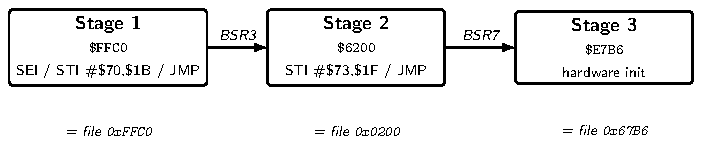
\includegraphics[width=0.35\textwidth]{title-graphic.pdf}}

\begin{document}

% ============================================================
\maketitle
\note{
Welcome.

I'm going to talk about what happened when I let Claude --- an LLM ---
loose on a real reverse-engineering problem. Specifically: build a Ghidra
processor module for a chip that Ghidra has never heard of, then use it to
take apart a 1997 modem firmware.

Two reasons this might be interesting at Congress, especially this year:

(1) The CCC audience is, correctly, sceptical of AI hype. I don't have
any hype to sell you. I have a four-day case study with both successes
and a substantive bug that needed a human to catch.

(2) The artefact is real. It's checked in, it has tests, and you can
download it tonight and feed your own L3902 firmware to it.

Talk is roughly 45 minutes. I'll save questions for the end.
}

% ============================================================
\section{Disclaimers}

\begin{frame}{What this talk is \emph{not}}
\begin{itemize}
  \item ``AI replaces reverse engineers.''
  \item ``You can prompt your way to a working tool.''
  \item ``LLMs are about to make Ghidra obsolete.''
  \item Vendor pitch. There is no product here. Just a git repo.
\end{itemize}
\vspace{0.5em}
\pause
\textbf{What it is:} four days of pair-programming with an LLM on a
specific RE task, with the receipts. Including the part where I got
something wrong and someone with grey hair fixed it.
\note{
Set expectations early. CCC audience is allergic to AI hype, with good
reason. I want to acknowledge that up front.

I'm not selling anything. The only thing I'm advocating for is: if
you're a reverse engineer and you're sceptical, don't dismiss this
without trying it. Form your scepticism from first-hand experience.

If you ARE running on hype, this talk should also slow you down. There
is a real failure mode in the middle of the story.

The "grey hair" thing is the German custom of trusting older technical
expertise --- this is for the German contingent. Mention it lightly.
}
\end{frame}

\begin{frame}{The deal}
\begin{itemize}
  \item Audience: you, sceptical.
  \item Subject: AI-assisted RE, on a real chip with real datasheets.
  \item Outcome metric: a working Ghidra module, a tested SLEIGH spec,
        and a 350-line analysis writeup. Or not. We'll see.
  \item Counterweight: the bug that proves the AI didn't really
        understand what it was doing.
\end{itemize}
\note{
Frame the rest of the talk: this is a single concrete case study.
Generalise from it cautiously, but it's at least one data point.

Audience may push back at the end. That's fine. I have specific things
I'll say worked and specific things I'll say didn't, and the receipts
are in the public repo.
}
\end{frame}

% ============================================================
\section{The artefact}

\begin{frame}{A piece of 1997 hardware}
\begin{columns}[T,onlytextwidth]
\column{0.55\textwidth}
\textbf{ELSA MicroLink 33.6 TQV}
\begin{itemize}
  \item German consumer modem, 1997
  \item 33.6 kbps V.34 + V.42bis + LAPM
  \item Class 2 fax (T.30)
  \item +V voice mode (V.253)
  \item H.324 video over POTS
\end{itemize}

\column{0.45\textwidth}
\textbf{Inside}
\begin{itemize}
  \item Rockwell L3902 MCU
  \item RC240VFC analog front-end
  \item 128 KiB external EPROM
  \item ${\sim}32$ KiB external SRAM
\end{itemize}
\end{columns}

\vspace{1em}
\textbf{Why this thing?} I had the firmware blob. The chip's CPU is
6502-derived but \emph{not} 6502, and Ghidra ships nothing for it.

\note{
Frame the artefact briefly. The audience here mostly grew up with
modems --- this is nostalgia hardware for them. That's fine.

Key non-obvious detail: Class 2 fax + voice + H.324. This isn't a basic
modem; it's a full V.253 voice modem, capable of fax sending/receiving
and video conferencing over POTS. That's a non-trivial firmware budget
in 128 KiB.

The "I had the firmware blob" — the audience will assume I dumped it
or downloaded it. Either way, neither shipping it nor asking how I got
it is the point. The point is the chip, which has zero open tooling.
}
\end{frame}

\begin{frame}{The CPU: Rockwell R65C19}
\begin{columns}[T,onlytextwidth]
\column{0.5\textwidth}
\textbf{Enhanced 6502}, late 1980s.\\[0.4em]
On top of stock 65C02:
\begin{itemize}
  \item 12 new bit-manip / branch ops
  \item 21 new arithmetic ops (\texttt{MPY}, \texttt{MPA},
        \texttt{NEG}, \texttt{ASR}, \texttt{ADD}, \dots)
  \item 10 threaded-code ops
        (\texttt{NXT}, \texttt{TIP}, \texttt{JPI}, \dots)
  \item 16-bit \texttt{W} reg (multiply accumulator)
  \item 16-bit \texttt{I} reg (Forth-style instruction pointer)
\end{itemize}

\column{0.5\textwidth}
\textbf{The trap nobody mentions}\\[0.4em]
Two addressing modes are silently redefined:
\begin{itemize}
  \item \texttt{(zp,X)} \;$\to$\; \texttt{(zp)}
  \item \texttt{(zp),Y} \;$\to$\; \texttt{(zp),X}
\end{itemize}
\vspace{0.5em}
Same opcodes. Different semantics.\\
\textit{Loading as 65C02 fails about 1\,KiB in.}
\end{columns}
\note{
The R65C19 is interesting because it's not "6502 with extra ops on the
side". The new ops use opcodes that 6502 NMOS marked illegal — fine.
But Rockwell also ALTERED two of the standard 6502 indirect modes.

The trap: if you load this firmware as 65C02, the disassembly looks
correct for the first few hundred bytes (no indirect ops), then
silently goes wrong. Everywhere there's a `(zp,X)` it should be a
`(zp)`. Branch targets are wrong, control flow is wrong, and you're
debugging a phantom.

Fixing this requires writing a SLEIGH processor spec from scratch.
Which is what this talk is about.
}
\end{frame}

\begin{frame}[fragile]{Banking}
The L3902 talks to its 128 KiB EPROM through 8 bank-select registers
at \texttt{\$0018-\$001F}. Each one maps a single 8 KiB physical bank
into one of eight 8 KiB windows in the CPU's 64 KiB view.
\vspace{1em}

\begin{lstlisting}[language=]
BSRn = | ES3 | ES2 | ES1 | ES0 | A16 | A15 | A14 | A13 |
         bit7  bit6  bit5  bit4  bit3  bit2  bit1  bit0
\end{lstlisting}

\vspace{0.4em}
\begin{itemize}
  \item \texttt{A13--A16}: 4 bits = 16 physical banks $\times$ 8\,KiB = 128\,KiB
  \item \texttt{ES0--ES3}: chip-select assertions (signal type, not address)
\end{itemize}
\vspace{0.3em}
\textbf{Hold this slide in your head.} I will get this part wrong and
have to come back to it.
\note{
This slide is foreshadowing. The BSR encoding turns out to be the
exact thing the AI got wrong, and we'll come back to it in detail. I
want the audience to see the encoding now so the later "I had it
backwards" lands harder.

The four address bits cover all of the EPROM. The four ES bits do NOT
contribute to the address — they're chip-select signals. This is
something a human RE engineer who's worked with banked memory before
would know instantly. The AI confidently invented a different model.
}
\end{frame}

% ============================================================
\section{The plan}

\begin{frame}{What I asked the LLM to do}
Roughly:
\begin{enumerate}
  \item Read the R65C19 datasheet. Build a SLEIGH spec covering the
        whole ISA, including the indirect-mode trap.
  \item Read the C40/L39 manual. Build the L3902-specific bits:
        peripheral symbols, vector table, memory map.
  \item Write a Ghidra loader that handles >64\,KiB banked images.
  \item Write tests: SLEIGH compile, opcode-decode fixture, end-to-end
        firmware import.
  \item Run it. Show me what the firmware does.
\end{enumerate}
\vspace{0.5em}
This is not ``one prompt.'' Over four days I sent maybe 30 messages.
\note{
The framing matters. I didn't open ChatGPT and ask "build a Ghidra
module for a Rockwell L3902". I structured the work as a sequence of
discrete tasks, each one verifiable.

Total interaction was maybe 30 messages over four sessions. Each
session ended with something runnable. That's the rhythm: AI does
boilerplate, you check the output, fix what's wrong, move on.

If you treat this as autonomous, you get plausible nonsense. If you
treat it as pair-programming with someone who works very fast and has
read every reference doc but has no judgement, you get a lot done.
}
\end{frame}

\begin{frame}{What the LLM had access to}
\begin{itemize}
  \item Three vendor PDFs (R65C19 data sheet, C40/L39 TRM, RC240VFC)
  \item The 128 KiB firmware blob
  \item A working Ghidra install at \texttt{/home/honx/ghidra}
  \item Shell, file editing, the SLEIGH compiler, headless analysis
  \item No internet. No prior code. No examples.
\end{itemize}
\vspace{0.5em}
The session was Claude Code (Anthropic's CLI agent). Same pattern
should work in any agentic setup with shell + file editing.
\note{
Important: this is local. The LLM had file/shell access but no web
access. It read the vendor PDFs through Anthropic's PDF tool, ran the
SLEIGH compiler on actual files, and ran Ghidra headless.

Why it matters: the audience may assume "the AI just looked up
existing R65C19 SLEIGH code online." It did not. There isn't any. The
spec was derived from reading 46-page R65C19 data sheet OCR, including
a 256-cell opcode matrix.

I'm using Claude Code specifically because it has good tool-use, but
the workflow generalises. Cursor, Aider, anything with shell + file
tools.
}
\end{frame}

% ============================================================
\section{Building the SLEIGH spec}

\begin{frame}{What SLEIGH is}
Ghidra's processor description language. Defines:
\begin{itemize}
  \item Endianness, address spaces
  \item Registers and flags
  \item Tokens (how opcodes are decomposed bit-by-bit)
  \item Constructors: ``these bytes mean this disassembly + this p-code''
\end{itemize}
\vspace{0.6em}
Built-in 6502 spec ships with Ghidra. \emph{Not} reusable here:
\texttt{(zp,X)} and \texttt{(zp),Y} are baked into the operand tables.
\vspace{0.3em}

The R65C19 spec is one self-contained file, $\sim$600 lines.
\note{
Quick orientation for people who haven't written SLEIGH. It's a small
domain-specific language for describing instruction sets. Pretty
declarative. Reasonably well-suited to LLM work because it's
mechanical: "this byte pattern means this mnemonic with these
operands."

Why I didn't @include the existing 6502 spec: the addressing-mode
remap is in the operand-resolution tables, which the 6502 spec
defines globally. Overriding them is messier than rewriting the
relevant constructors.

600 lines is small for an ISA spec. The bulk is the instruction
constructors; tokens and macros are maybe 80 lines.
}
\end{frame}

\begin{frame}[fragile]{Sample constructor: \texttt{STI \#imm,\$zp}}
\textbf{The R65C19's three-byte store-immediate-to-zero-page op:}
\begin{lstlisting}[language=sleigh]
# STI ($B2): 3 bytes - op, immediate value, ZP destination address.
:STI "#"imm8b, imm8 is op=0xB2; imm8b; imm8
{
    local addr:2 = imm8;
    *:1 addr = imm8b:1;
}
\end{lstlisting}
\vspace{0.4em}
Read it left to right:\\
``\texttt{STI} \#\textit{value}, \textit{address} matches when the opcode
byte is \texttt{0xB2}, followed by an 8-bit value, then an 8-bit
address. P-code: write the value to that address.''
\vspace{0.4em}

181 occurrences in the firmware. Rockwell did not skimp on this op.
\note{
Show one constructor in detail so the audience sees what SLEIGH looks
like. Pick STI because it's the most-used R65C19 extension.

Bit of pedagogy: SLEIGH constructors have three parts. The display
format string defines what gets printed in the listing. The
bit-pattern match defines when this constructor fires. The p-code
semantics block defines what the instruction actually does.

The token "imm8b" exists separately from "imm8" because SLEIGH won't
let two operands of the same token type appear in one instruction. So
the spec defines a parallel one-byte token for the second operand.
That's a minor SLEIGH-grammar gotcha that the LLM did stumble on once
and had to fix. Mention it briefly.
}
\end{frame}

\begin{frame}[fragile]{Indirect-mode remap}
\textbf{The thing 65C02 gets silently wrong on R65C19:}
\begin{lstlisting}[language=sleigh]
# OP1 = operand class for cc=01 ALU instructions.
#   bbb=0  (zp)         R65C19 zero-page indirect (was (zp,X) on 6502)
#   bbb=4  (zp),X       R65C19 zp indirect, post-indexed by X (was (zp),Y)
OP1: (imm8)     is bbb=0; imm8        { addr:2 = imm8; tmp:2 = *:2 addr;
                                        export *:1 tmp; }
OP1: (imm8),X   is bbb=4 & X; imm8    { addr:2 = imm8; tmp:2 = *:2 addr;
                                        tmp = tmp + zext(X); export *:1 tmp; }
\end{lstlisting}
\vspace{0.3em}

Two slots in the operand table that the LLM had to flip from the
stock 6502 versions. Without this, every \texttt{LDA (\$xx),X} in the
firmware decodes as \texttt{LDA (\$xx),Y} --- silently wrong.
\note{
This is the slot-flip that was the whole reason to write a custom
spec. Show it.

This is the kind of thing where the LLM did well: it had read both the
R65C19 datasheet's "instructions changed" table and the stock 6502
spec, and it correctly identified that the only way to express the
remap was to redefine OP1's bbb=0 and bbb=4 entries.

Mechanical, well-specified, the kind of work LLMs are good at.
}
\end{frame}

\begin{frame}{The opcode matrix}
The R65C19 datasheet has a 16$\times$16 opcode matrix. 256 cells, each
labelled with mnemonic + addressing mode + cycle count.\\[0.4em]

The LLM's job: read the matrix from a 1992 photocopy quality PDF,
expand each cell into a SLEIGH constructor.\\[0.4em]

\textbf{What worked:}
\begin{itemize}
  \item All 256 opcodes decoded correctly --- 0 unknown mnemonics in the firmware.
  \item Mnemonic lookup, encoding fields, byte counts: all OCR'd cleanly.
\end{itemize}

\textbf{What didn't:}
\begin{itemize}
  \item Three opcodes the LLM couldn't read confidently:
        \texttt{JPI}, \texttt{ADD zp}, \texttt{ADD zp,X}.\\
        Documented as ``unknown'' in \texttt{open-points.md}. None
        appear in the reference firmware, so the gap doesn't bite.
\end{itemize}
\note{
Be honest about the OCR step. It worked, but not perfectly. The LLM
was conservative: when it couldn't read a cell with confidence, it
flagged it and kept going.

That's good behaviour. The alternative — guessing — would have
produced code that disassembled wrongly. Having it be honest about
the OCR confidence level was important.

The three missing opcodes are real gaps but turn out not to matter
for this firmware. We verified that with a static scan after the fact.
If a future user runs the spec on a R65C19 image that uses JPI, they
get an "unknown opcode" mark and can extend the spec.
}
\end{frame}

% ============================================================
\section{The loader and the test suite}

\begin{frame}{Loader: banked memory}
Java loader, $\sim$150 lines. Recognises an L3902 firmware image by
size constraint (multiple of 8\,KiB up to 512\,KiB) and:
\begin{itemize}
  \item Maps the first 64\,KiB at \texttt{\$0000-\$FFFF} as ROM
  \item Layers uninitialised blocks for the on-chip I/O, RAM pages, CRC
  \item Reads the reset vector at \texttt{\$FFFE} and creates a
        \texttt{\_reset} function there
  \item For images $>$64\,KiB, drops each additional 64\,KiB chunk in
        as a \texttt{BANK\_HIGH\_n} overlay block
\end{itemize}
\vspace{0.6em}
Bank-aware cross-references --- ``after this \texttt{STI \#imm,\$1B},
\texttt{\$6200} reads from \texttt{file:0x0200}'' --- are
\textbf{not} implemented.\\
That's listed under open points.
\note{
The loader is the least interesting part of the work. It's
boilerplate Java that walks the bytes and creates Ghidra memory
blocks. LLM did this well because there are 50 example loaders in
Ghidra's source tree and the API is stable.

Caveat: the bank-aware cross-referencing IS the hard part, and it's
NOT implemented. Today, when Ghidra encounters an STI immediate
followed by a JMP to a bank-mapped address, it disassembles both
correctly but doesn't model the bank switch — so it follows the JMP
into whatever bytes were there before the switch.

Building a bank-aware analyser would be a serious piece of work. It's
the kind of thing where an LLM gets you 80% of a sketch and a human
finishes the engineering. It's on the open-points list.
}
\end{frame}

\begin{frame}[fragile]{Tests}
\textbf{Three of them, all green, all run in CI.}
\begin{itemize}
  \item \texttt{test\_01\_sleigh\_compiles.sh} --- recompile spec,
        fail on errors or unexpected warnings.
  \item \texttt{test\_02\_opcode\_decode.sh} --- generate a 64\,KiB
        synthetic fixture with 43 hand-picked opcodes, import,
        assert that each address disassembles to the expected mnemonic.
  \item \texttt{test\_03\_e2e\_firmware.sh} --- import the real ELSA
        firmware, run auto-analysis, assert on 16 invariants.
\end{itemize}
\begin{lstlisting}[language=]
=== test_01_sleigh_compiles.sh ===
  PASS SLEIGH spec compiles cleanly (2 warnings, 7461 byte .sla)
=== test_02_opcode_decode.sh ===
  PASS 43 opcode expectations satisfied
=== test_03_e2e_firmware.sh ===
  PASS 16 e2e assertions satisfied against the reference firmware
All 3 test(s) passed
\end{lstlisting}
\note{
This is a part of the workflow that I think is underappreciated. LLMs
write tests well — if you ask them to. They will happily not write
any tests if you don't.

The three tests cover three failure modes. Spec broken: test one
catches it. One opcode misencoded: test two catches it. Real-world
disassembly drifting: test three catches it.

The opcode-decode test surfaced two real bugs while I was writing it:
the unconditional branch in the fixture meant later opcodes weren't
linearly reachable (had to disassemble each address explicitly), and
the bitindex display format wasn't what I'd guessed it would be.
Tests catching test bugs early — fine, that's what tests are for.
}
\end{frame}

% ============================================================
\section{The analysis}

\begin{frame}[fragile]{First decode}
\textbf{Reset vector:} file \texttt{0xFFFE/F} = \texttt{c0 ff} → reset target \texttt{\$FFC0}.\\
\textbf{Disassembly at \$FFC0:}
\begin{lstlisting}[language=disasm]
$FFC0  78           SEI                    ; mask all IRQs
$FFC1  B2 70 1B     STI #$70, $1B          ; BSR3 := $70 - bank-switch
$FFC4  4C 00 62     JMP $6200              ; jump into newly-mapped bank
\end{lstlisting}
\vspace{0.5em}

\textbf{This is the moment the spec ``works.''}
\begin{itemize}
  \item Three instructions disassembled cleanly.
  \item One of them is the R65C19 \texttt{STI} extension that no
        stock 6502 spec can decode.
  \item Auto-analysis finds 204 functions in 4 seconds.
\end{itemize}

\note{
This is the demo moment. The first three instructions of the firmware
include the R65C19 extension we wrote SLEIGH for. If the spec were
broken, the disassembly would be visibly wrong here.

204 functions in 4 seconds is Ghidra's auto-analysis. That's not
"the LLM understood the firmware" — that's "Ghidra's analyser was
able to follow flow and identify subroutines, given a working
processor module."

For a sceptical audience, this is where the talk says "the spec
demonstrably works on real input." The rest of the talk is what we
USE the working spec to learn.
}
\end{frame}

\begin{frame}{What the firmware does, by string evidence}
The image carries its own functional spec, in printable strings. The
LLM dumped them, grouped them, and wrote them up.\\[0.6em]

\begin{description}\itemsep0.2em
  \item[\texttt{(C) ROCKWELL} / \texttt{ELSA Aachen}] branding (1997-07-18 build)
  \item[\texttt{V42bis}, \texttt{TxSymRa Bd}, \texttt{TxPrecoding}, \texttt{V34PwrRed}\dots] V.34 / V.42bis stats labels
  \item[\texttt{ROCKWELL;ADPCM;16}] non-standard voice-mode codec
  \item[\texttt{OK}, \texttt{CONNECT}, \texttt{NO CARRIER}, \texttt{DIAL LOCKED}\dots] AT result codes (Hayes/V.250)
  \item[\texttt{+FCON}, \texttt{+FHNG}, \texttt{+FDIS}, \texttt{+FCFR}, \texttt{+FNSC}\dots] Class 2 fax (T.30)
  \item[\texttt{NO H324 DETECTED}] H.324 video conferencing
  \item[\texttt{+VCON}] V.253 voice connection
  \item[\texttt{Konfiguration:}, \texttt{RX-Gain:}, \texttt{Werte des fernen Modems}] German diagnostic UI
\end{description}
\note{
Strings are the cheap part of RE — they tell you, for free, what the
firmware claims to do. The LLM categorised these from a flat list of
600+ strings.

This is honest pattern-matching. The LLM didn't "understand" what
T.30 is — it labelled the +F* strings as fax response codes because
that's what they are in the standard, and an LLM has read the
standard. That's appropriate use of the model's prior.

Important call-out: the same firmware blob services three SKUs
(14.4TQ, 28.8TQ, 33.6TQ). Single image, three product configurations
keyed off some flag.
}
\end{frame}

\begin{frame}[fragile]{Architecture, by code}
\textbf{Trampoline-driven dispatch.}\\
204 functions, 2179 instructions in the boot-time view. Many follow a
6-byte template:\\[0.6em]

\begin{lstlisting}[language=disasm]
LDY $85
RND
STI #$03, $41           ; command opcode
STI #$12, $40           ; sub-command
JSR $E81B               ; central dispatcher
RTS
\end{lstlisting}
\vspace{0.5em}

\begin{itemize}
  \item One stub per AT command. (\texttt{\$41},\texttt{\$40}) = command pair.
  \item Dispatcher at \texttt{\$E81B} does the table lookup once, for everyone.
  \item \texttt{STI} alone accounts for 8.3\% of the instruction stream.
\end{itemize}
\note{
This is the architectural insight: the firmware is built around a
single dispatcher with dozens of tiny per-command stubs. Classic
Rockwell modem-firmware style — the dispatch table is in ROM, and
everything else is parameter setup.

8.3% STI density is unusual. For a stock 6502 firmware that number
would be 0% (no STI at all). For R65C19 with this dispatch style it's
the third-most-common instruction.

Bit-manipulation density (BAR/BAS/SBA/RBA/BBR/BBS/SMB/RMB) is 8.6%.
That's also unusual. The firmware spends a lot of time setting and
reading individual bits in control registers — which makes sense for
something whose job is talking to peripherals.
}
\end{frame}

% ============================================================
\section{The bug}

\begin{frame}[standout]
The bug.\\[0.5em]
\large{Where the LLM's confident wrongness met a human reviewer.}
\note{
This is the part I wanted to do justice to. The talk would be cheap if
I just showed everything that worked. The real lesson is in the place
the AI got something wrong, sounded confident about it, and a human
caught it.

Pause here. Slow down. The next four slides are the most important
ones in the talk for a sceptical audience.
}
\end{frame}

\begin{frame}{What the LLM said}
After analysing the boot stub the LLM wrote, in the analysis document:

\vspace{0.7em}
\begin{quote}
\itshape
``The 128 KiB image is laid out so that \textbf{the first 64 KiB is
what the L3902 sees while only ES0 is active}, and the second 64 KiB
is what it sees once ES1, ES2 and ES3 are also asserted. \dots The
boot stub bank-switches BSR3 to expose chip-2 in the \$6000-\$7FFF
window, then jumps to \$6200.''
\end{quote}

\vspace{0.7em}
This is the ``two physical chips'' theory. It is plausible, parses
the BSR write, sounds technically literate.\\
\textbf{It is also wrong.}
\note{
Show the actual quote from the analysis writeup as it stood after the
LLM's first pass. This is what got committed to the repo before
review.

Why it sounds plausible: it parses the BSR encoding, it explains where
the second 64 KiB comes from, it accounts for the chip-select bits.
It's an internally-consistent model.

Why it's wrong: it ignores the part of the BSR encoding that says
A13-A16 is FOUR bits, not three. Four bits = 16 banks. 16 banks of
8 KiB = 128 KiB. The whole EPROM, addressed by A13-A16 alone.

The LLM read the BSR encoding correctly, then constructed a system
model that didn't match the encoding it had just read. That's a
specific failure mode worth naming: confident pattern-fitting without
checking.
}
\end{frame}

\begin{frame}[fragile]{What the human said}
Eight hours after the analysis was committed, a friend with hands-on
modem RE experience read it and emailed:

\vspace{0.5em}
\begin{quote}
\small\itshape
\texttt{FFC1 B2 70 1B STI \#70, \$1B}\\
\texttt{; Bank Select 3}\\
\texttt{;   01110000}\\
\texttt{;     6000-7FFF -> ROM 0000-1FFF}\\[0.5em]

d.h. bei \texttt{6200h} finde ich dann den Code, der im Binärfile bei
\texttt{0200} steht. Das erklärt vieles.
\end{quote}

\vspace{0.6em}
``So at \texttt{6200h} I find the code that's at \texttt{0200} in the
binary file. That explains a lot.''
\note{
Read the friend's email. Slow down. This is what good RE review
looks like.

He didn't say "you're wrong". He said "here's the encoding, here's
what it means, here's where the code actually is". One line.

The encoding-decoding is unambiguous: BSR3 equals hex seventy, in
binary that's zero-one-one-one zero-zero-zero-zero. The four low
bits, which are A13 through A16, are all zero — meaning physical
bank zero. Physical bank zero of a 128 KiB EPROM is file offsets
zero through 0x1FFF. So logical 6200 hex maps to file 0x0200,
period.

The LLM's two-chips model said 6200 hex maps to file 0x10200. The
reviewer checked. It doesn't.
}
\end{frame}

\begin{frame}[fragile]{What was actually at file \texttt{0x0200}}
Eight bytes:
\vspace{0.4em}
\begin{lstlisting}[language=disasm]
file 0x0200:  B2 73 1F  4C B6 E7
              STI #$73, $1F           ; BSR7 := $73 - second-stage bank-switch!
              JMP $E7B6               ; into the newly-mapped bank
\end{lstlisting}
\vspace{0.4em}

\textbf{It's a second boot stub.}\\[0.4em]

\begin{itemize}
  \item Stage 1 (\$FFC0): bank-switch \texttt{BSR3}, jump to \$6200.
  \item Stage 2 (\$6200, = file \texttt{0x0200}): bank-switch \texttt{BSR7}, jump to \$E7B6.
  \item Stage 3 (\$E7B6, = file \texttt{0x67B6}): the \emph{real} hardware initialiser.
\end{itemize}
\vspace{0.4em}

A three-stage boot trampoline, hidden in plain sight. The LLM never
saw it because its memory model said $6200$ wasn't where the bytes
\texttt{B2 73 1F} lived.
\note{
Walk through the chain. This is the key technical content.

When you do follow the chain correctly, you discover the firmware has
a beautifully economical three-stage boot. Each stage is two
instructions before its `JMP`. Each stage bank-switches its successor
into view, then jumps. The third stage finally programs all eight BSRs
to the runtime memory map.

This is GOOD firmware engineering, the kind you only see when every
byte of ROM costs money. It's also the kind of structural insight the
LLM had no chance of finding because its starting model was wrong.

This was not a small bug. It changed our entire reading of the
firmware. Before the correction: "first 64 KiB is data, second 64 KiB
is code." After: "single 128 KiB image, three-stage trampoline, all
the code lives in low banks."
}
\end{frame}

\begin{frame}{The lesson}
The LLM had read:
\begin{itemize}
  \item The full BSR encoding.
  \item The 128 KiB file size.
  \item The L39 TRM's ``up to 512 KiB external memory'' claim.
\end{itemize}
\vspace{0.4em}

It had \emph{enough information} to derive the right model.\\
It instead constructed a confident, plausible, wrong one.\\[0.6em]

\textbf{Specific failure mode:} pattern-fit a coherent narrative around
incomplete reasoning, present it as established fact.\\[0.4em]

\textbf{Specific corrective:} a human with hands-on experience reading
the encoding from the bit pattern and saying ``no, that's bank zero,
the file offset is \texttt{0x0200}.''\\[0.6em]

\emph{The bit pattern was visible to both of us. Only one of us read
it correctly.}
\note{
Be precise about what the failure was. Not "the LLM hallucinated".
Not "the LLM didn't have enough information". The information was
all there. The LLM constructed a plausible-but-wrong model and
wrote it up as fact.

This is the failure mode that every serious AI user has to learn to
recognise. The LLM's outputs are calibrated for plausibility, not
correctness. When the two diverge, plausibility wins, until a human
intervenes.

The corrective is not "trust the human more". The corrective is to
have the LLM and the human reading the same artefact, and to send
the LLM back to the artefact with a specific question whenever
something doesn't add up.

In this case the friend didn't even need to know the L3902 to be
right. He just READ THE ENCODING. The LLM had read it too. The
difference is the friend then USED what he'd read to derive the
answer. The LLM had moved on.
}
\end{frame}

\begin{frame}{What got fixed}
After the correction, in one round of edits:
\begin{itemize}
  \item Analysis writeup rewritten ($\sim$70 lines changed) with the
        correct three-stage boot model.
  \item \texttt{docs/architecture.md} gained a ``Banking is not in the
        SLEIGH spec'' section explaining what SHOULD model banking
        (loader + analyser, not slaspec).
  \item \texttt{docs/open-points.md} BSR-aware-analysis bullet
        strengthened with the boot trampoline as motivation.
  \item E2E test grew 7 new assertions covering the second and third
        stages and the runtime IRQ vector table.
\end{itemize}
\vspace{0.6em}

The repo now has \emph{both} the original mistake (in git history) and
the correction (with attribution in the commit message).
\note{
Show what shipped after the correction. The point is that the
correction was small, surgical, and produced a better artefact.

The git history matters. Both commits are in the repo. Anyone who
clones it can see the wrong version, the email-driven correction, and
the new tests that prevent the same kind of mistake from recurring
silently.

This is what "AI in the loop" should look like in practice. Not
"AI replaces human review". "AI does work fast, human reviews,
mistakes get pushed back, repo gets better."

But — and this is the next slide — the same human came back two days
later with a SECOND correction.
}
\end{frame}

% ============================================================

\begin{frame}{And then \dots\ a second email}
Two days after the analysis was committed and corrected, a follow-up
arrived with a screenshot. One table:\\[0.4em]

\centering
\small
\begin{tabular}{lcccc}
\toprule
\textbf{Bank} & \textbf{Cfg1} & \textbf{Cfg2} & \textbf{Cfg3} & \textbf{Cfg4} \\
\midrule
B0 (\$0200)   & ROM0  & ROM8 & ROM10 & ROM18 \\
B2 (\$2000)   & ROM2  & ROMA & ROM12 & ROM1A \\
B4 (\$4000)   & ROM4  & ROMC & ROM14 & ROM1C \\
B6 (\$6000)   & ROME  & INX  & ROM16 & ROM1E \\
\midrule
B8 (\$8000)   & RAM0  & RAM0  & RAM0  & RAM0 \\
BA (\$A000)   & RAM1  & RAM1  & RAM1  & RAM1 \\
BC (\$C000)   & RAM2  & RAM2  & RAM2  & RAM2 \\
BE (\$E000)   & ROM6  & ROM6  & ROM6  & ROM6 \\
\bottomrule
\end{tabular}
\\[0.6em]

``\itshape Nach dem Reset wird die Konfiguration Cfg2 aktiviert.''
\note{
Read the table. Slow.

This is the actual runtime banking model the firmware uses. Not "the
firmware reprograms BSRs whenever it needs to" — the firmware switches
between FOUR named, hand-tuned configurations. Three of the four BSR
windows always hold RAM. One always holds the persistent code bank.
The four lower windows swap between four named codings — Cfg1 through
Cfg4.

After reset, Cfg2 is active. That matches what the third boot stub
writes — and once you read the table back against the disassembly,
the eight STI writes in the third stub *exactly* establish Cfg2.

I had described the third stub correctly at the byte level. I had
called the resulting state "the runtime memory map". I had not
recognised that the firmware authors had a four-state design with
named transitions between them.
}
\end{frame}

\begin{frame}{What the second correction added}
\textbf{Before:} ``a single runtime memory map after init.''\\[0.3em]
\textbf{After:} ``four named configurations the firmware switches between.''\\[0.6em]

\begin{itemize}
  \item There are four functions called \texttt{switch\_rom\_cfg1()}
        through \texttt{switch\_rom\_cfg4()}. Each writes the eight BSR
        values for one configuration.
  \item Three of the BSR windows are \emph{always} the same: 24\,KiB
        of external SRAM at \$8000-\$DFFF, plus a persistent code bank
        ROM6 at \$E000-\$FFFF.
  \item The lower four windows (\$0200-\$7FFF) swap between four ROM
        groupings. The whole 128\,KiB EPROM gets used: 8\,KiB of code
        always present, plus 32+24+24+32\,KiB swapped in by config.
  \item Reset puts the chip in Cfg2.
\end{itemize}

\vspace{0.4em}
\textbf{What this corrects:} my ``runtime memory map'' was the
post-reset Cfg2 state. I'd missed that there are three other states
the firmware also uses.
\note{
Architectural insight that the AI didn't get to on its own. The
firmware authors had partitioned the address space into:
- a fixed code+RAM region (always present, contains the dispatcher)
- a dynamic ROM region that swaps between four named contents

That's a clean engineering pattern, and it explains things I'd
previously written off as "weird" — like why the AT result codes (in
Cfg3) were in a different physical region than the fax responses (in
Cfg4). The command parser switches configurations based on which
subsystem the AT command targets.

The bank-aware-analyser story I'd told earlier — "track every STI
write to a BSR" — was also wrong-ish. The realistic shape of that
analyser is: recognise calls to a small number of named
configuration-switch functions, and follow the implied overlay change.
Much more tractable than tracking arbitrary BSR writes, and it matches
how real firmware is actually written.
}
\end{frame}

\begin{frame}{Two corrections, one lesson}
\begin{itemize}
  \item \textbf{Round 1 (the BSR encoding):} I had ``two physical
        chips''. He had ``read the bit pattern.''
  \item \textbf{Round 2 (the four configurations):} I had ``one
        runtime memory map''. He had ``four named configurations the
        firmware actually uses.''
\end{itemize}
\vspace{0.6em}

In both rounds, the corrective came from someone who had \emph{worked
on this kind of firmware before}.\\[0.4em]

The LLM had read a 119-page L39 manual and a 46-page R65C19 datasheet.\\
What it didn't have was the embedded engineer's reflex of asking,
``what does the firmware author's mental model look like?''
\note{
The deeper observation. The first correction was about an encoding
detail. The second was about a programmer's *mental model* of their
own system. The LLM doesn't have any priors about how embedded
engineers structure firmware — it just has the bytes and the
datasheet.

For people in the audience who write firmware: this is the part of
your job an LLM is not going to take. You build mental models of
machines you understand from the inside. The LLM operates on bytes
and documentation; it's good at that, but the synthesis you do — "in
1997, an embedded engineer with 24 KiB of code budget per
configuration would..." — is not coming from a model trained on
GitHub.

For people sceptical of AI in RE: this is the failure mode you should
be sceptical of. Don't let the LLM produce a "complete picture" you
haven't checked against the priors of someone who's done this work
before.
}
\end{frame}

% ============================================================
\section{Honest assessment}

\begin{frame}{What worked well}
\begin{itemize}
  \item \textbf{SLEIGH grammar and constructors} --- mechanical,
        well-specified, large existing corpus. LLM strength.
  \item \textbf{Loader boilerplate} --- 50 example loaders in Ghidra
        source. LLM had absorbed the API.
  \item \textbf{Test scaffolding} --- shell drivers, headless scripts,
        fixture generation. Mostly boilerplate.
  \item \textbf{Documentation at multiple levels} --- overview,
        usage, architecture, open-points. Tedious for humans, fast
        for an LLM.
  \item \textbf{Refactoring under spec} --- ``move this to a separate
        cspec file,'' ``rename \texttt{I} to \texttt{Iflag} to avoid
        the threaded-code reg collision''. Mechanical.
\end{itemize}
\note{
Be specific about what the LLM contributed real value to. These are
all tasks where the LLM's training has seen many similar examples,
and the work is mostly applying known patterns to a new instance.

Documentation is underrated. I now have FOUR documents covering this
project at different levels, plus a 350-line firmware analysis. I
would not have written that documentation by hand. Not in four days,
maybe not ever.

Tests too. Without prompting, the LLM defaulted to "no tests". With
explicit asks for tests, it produced a respectable suite. That's a
prompting issue, not a capability issue.
}
\end{frame}

\begin{frame}{What didn't work well}
\begin{itemize}
  \item \textbf{Confident speculation about hardware semantics} ---
        the BSR bug is the canonical example.
  \item \textbf{Inferring meaning from incomplete OCR} --- three
        opcodes silently dropped because the matrix scan wasn't
        clean. Honest about the gap, but a human would have asked for
        a higher-resolution scan.
  \item \textbf{Cross-bank reasoning} --- when the firmware's logical
        \$6200 reads from a different file offset than the user
        thinks, the LLM's mental model drifted before it had a chance
        to be wrong on paper.
  \item \textbf{``Verifying'' without actually verifying} --- the LLM
        sometimes claimed it had checked something it had only
        plausibility-tested. Pre-commit, before the friend's email.
\end{itemize}
\note{
Counterweight slide. These are the real limitations, not strawmen.

The "verifying without verifying" one is worth dwelling on. LLMs will
say "I confirmed X" when what they actually did was "I generated text
asserting X, with no evidence-gathering step". Detecting this requires
either (a) the human asking "show me the evidence", or (b) automated
tests that fail when the claim is wrong. Both are valuable.

This is also why the test suite matters. The end-to-end test catches
disassembly drift. If a future "improvement" to the spec broke the
boot stub disassembly, the e2e test would fail.
}
\end{frame}

\begin{frame}{The collaboration model}
\begin{columns}[T,onlytextwidth]
\column{0.5\textwidth}
\textbf{Human}
\begin{itemize}
  \item Picks the target.
  \item Defines what ``done'' means.
  \item Verifies hardware semantics.
  \item Reads the bit patterns.
  \item Reviews the bigger claims.
\end{itemize}

\column{0.5\textwidth}
\textbf{LLM}
\begin{itemize}
  \item Reads the datasheet pages.
  \item Writes the boilerplate.
  \item Writes the tests.
  \item Writes the docs.
  \item Refactors on request.
  \item Surfaces inconsistencies.
\end{itemize}
\end{columns}

\vspace{1.2em}
\textbf{What this is not:} hand-the-LLM-a-PDF, get-a-Ghidra-module-back.

\textbf{What this is:} pair-programming with someone who works very
fast, has read every reference doc, and has no engineering judgement.
You provide the judgement.
\note{
Land the pitch. The collaboration model is the substance of the talk.

The point is: this isn't autonomous coding. It isn't replacement of
the engineer. It's a force multiplier on the parts of the work that
LLMs are good at, paired with a human doing the parts they're bad at.

For a sceptical audience: this is consistent with what your scepticism
says LLMs can't do. The trick is identifying which parts of a project
fit the LLM strength profile and which need real engineering
judgement.

If you do that mapping correctly, the throughput is genuinely several
times what a human alone would deliver. If you don't, you get
plausible nonsense fast.
}
\end{frame}

% ============================================================
\section{The artefact}

\begin{frame}{What's in the repo}
\centering
\textbf{\large github.com/honx/rockwell\_l39\_ghidra}\\[0.6em]
\begin{itemize}\itemsep0.3em
  \item Full Ghidra processor module (drop-in)
  \item SLEIGH spec, $\sim$600 lines, all R65C19 ISA
  \item Java loader for banked images
  \item Three tests, all green, runnable
  \item Four docs (overview/usage/architecture/open-points)
  \item 350-line analysis of the ELSA firmware
  \item Reference firmware excluded by \texttt{.gitignore} (not ours
        to redistribute)
\end{itemize}
\vspace{0.8em}
Apache 2.0. Patches welcome. The bug history is in the git log; if
you want to see what the LLM got wrong before review, look at commit
\texttt{20026e9\^{}}.
\note{
Land where to find it. Repo is small, self-contained, and includes
the wrong-then-right history so anyone can audit.

The bug commit message is honest about what changed and why. Reading
it is itself an example of the kind of human-AI collaboration the talk
is arguing for.
}
\end{frame}

\begin{frame}{Closing}
\begin{itemize}
  \item LLM-assisted RE works on real targets, with caveats.
  \item The caveats include a real failure mode that needs human
        review.
  \item ``Real'' here means: tested, documented, on a chip Ghidra had
        never heard of, four days from blank page to disassembled
        firmware.
\end{itemize}
\vspace{0.8em}
If you remember one thing:
\begin{quote}
\itshape
The LLM is a fast junior collaborator with no engineering judgement.\\
Treat it like one and it produces good work.\\
Treat it like a senior engineer and it ships confident bugs.
\end{quote}
\note{
Closing line. Pause, then open Q\&A.

If asked: yes, I'm aware this is just one case study. No, I don't
have benchmarks. The repo and the test suite are the falsifiable
artefact. Anyone who wants to disprove the case study can fork the
repo, propose a fix, and see whether the tests still pass.
}
\end{frame}

\begin{frame}[standout]
Questions?\\[1em]
\large \emph{honx@thinventions.de}\\
\large \emph{github.com/honx/rockwell\_l39\_ghidra}
\note{
Q\&A. Anticipated questions:

Q: What model? Sonnet 4.6 / Opus 4.7. The session was Claude Code in
auto mode. The work is reproducible with any agentic LLM that has
shell + file tools.

Q: How much did you spend? Honestly, low single-digit dollars on
inference cost over four sessions. The economics are favourable for
this kind of focused work.

Q: Could you have done this without an LLM? Yes, in maybe 4 weeks of
part-time evening work. With the LLM it was 4 days. The hard
intellectual content (the bug-finding, the BSR encoding correction)
was still human work.

Q: What about adversarial use? Out of scope. RE is dual-use; this
talk is on the defensive/research side.

Q: Bank-aware analyser, when? PR welcome. It's the obvious next
step.
}
\end{frame}

\end{document}
